%%%%%%%%%%%%%%%%%%%%%%%%%%%%%%%%%%%%%%%%%
% Developer CV
% LaTeX Template
% Version 1.0 (28/1/19)
%
% This template originates from:
% http://www.LaTeXTemplates.com
%
% Authors:
% Jan Vorisek (jan@vorisek.me)
% Based on a template by Jan Küster (info@jankuester.com)
% Modified for LaTeX Templates by Vel (vel@LaTeXTemplates.com)
%
% License:
% The MIT License (see included LICENSE file)
%
%%%%%%%%%%%%%%%%%%%%%%%%%%%%%%%%%%%%%%%%%

%----------------------------------------------------------------------------------------
%	PACKAGES AND OTHER DOCUMENT CONFIGURATIONS
%----------------------------------------------------------------------------------------

\documentclass[8pt]{developercv} % Default font size, values from 8-12pt are recommended

%----------------------------------------------------------------------------------------



\begin{document}

%----------------------------------------------------------------------------------------
%	TITLE AND CONTACT INFORMATION
%----------------------------------------------------------------------------------------

\begin{minipage}[t]{0.50\textwidth} % 45% of the page width for name
	\vspace{-\baselineskip} % Required for vertically aligning minipages

	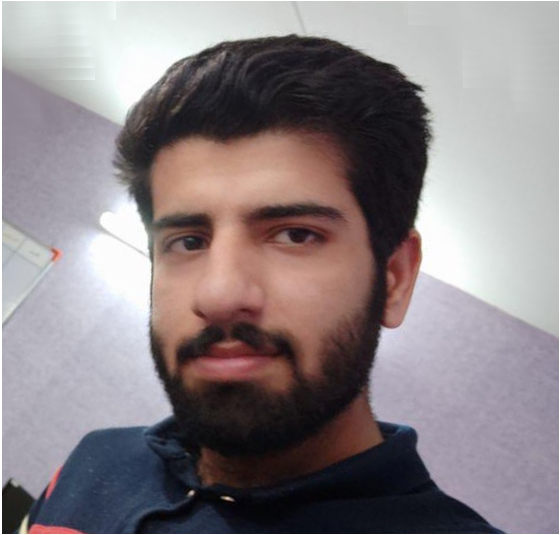
\includegraphics[width=0.4\textwidth]{me.png}

	\vspace{5pt}

	% If your name is very short, use just one of the lines below
	% If your name is very long, reduce the font size or make the minipage wider and reduce the others proportionately
	\colorbox{black}{\Huge{\textcolor{white}{Morteza Jalambadani}}} % First name
	
%	\colorbox{black}{{\Large\textcolor{white}{Jalambadani}}} % Last name
	
	\vspace{5pt}

	{\LARGE {\color{gray}Developer and Data scientists}} % Career or current job title
\end{minipage}
\begin{minipage}[t]{0.25\textwidth} % 27.5% of the page width for the first row of icons
	\vspace{-\baselineskip} % Required for vertically aligning minipages
	\vspace{50pt}

	% The first parameter is the FontAwesome icon name, the second is the box size and the third is the text
	% Other icons can be found by referring to fontawesome.pdf (supplied with the template) and using the word after \fa in the command for the icon you want
	\icon{Phone}{12}{\href{tel:+98 939 166 1481}{+98 939 166 1481}}\\\\
	\icon{At}{12}{\href{mailto:morteza@jalambadani.ir}{Morteza@Jalambadani.ir}}\\\\
	\iconWhite{Terminal}{5}{\href{http://Jalambadani.ir}
	{Jalambadani.ir}}\\\\

\end{minipage}
\begin{minipage}[t]{0.25\textwidth} % 27.5% of the page width for the second row of icons
	\vspace{-\baselineskip} % Required for vertically aligning minipages
	\vspace{50pt}

	% The first parameter is the FontAwesome icon name, the second is the box size and the third is the text
	% Other icons can be found by referring to fontawesome.pdf (supplied with the template) and using the word after \fa in the command for the icon you want
    \icon{Google}{12}{\href{mailto:morteza.j8@gmail.com}{Morteza.J8@gmail.com}}\\\\
	\icon{Github}{12}{\href{https://github.com/Morteza-j8}{github.com/Morteza-j8}}\\\\
	\iconWhite {StackOverflow}{5}{\href{https://stackoverflow.com/users/5919568/morteza-jalambadani?tab=profile}{morteza-jalambadani}}\\\\
	%\icon{Telegram}{12}{\href{https://t.me/morteza_jalambadani}{@Morteza_Jalambadani}}\\
\end{minipage}

\vspace{0.5cm}

%----------------------------------------------------------------------------------------
%	INTRODUCTION, SKILLS AND TECHNOLOGIES
%----------------------------------------------------------------------------------------
\noindent\rule{\textwidth}{1pt}

\center {\cvsect{About Me}}
\vspace{15pt} % Required for vertically aligning minipages

\begin{minipage}[t]{0.5\textwidth} % 40% of the page width for the introduction text
	\vspace{-\baselineskip} % Required for vertically aligning minipages

	\Large {
	\begin{itemize}
		\item {Born In \textbf{August 12, 1996}}
		\item {Live in
		\href{https://www.google.com/maps/place/Mashhad,+Razavi+Khorasan+Province,+Iran/@36.2976014,59.5092469,12z/data=!3m1!4b1!4m5!3m4!1s0x3f6c911abe4131d7:0xc9c57e3a9318753b!8m2!3d36.2619922!4d59.6173096}
		{\textbf{Mashhad}}}
		\item {Marital Status: \textbf{Single} }
		\item {Military Service: \textbf{Education} \normalsize{\textsc{(until 2022)}} }
		\item {Developer Experience: \textbf{ 5 Years}  }
	\end{itemize}
	}

\end{minipage}
\hfill % Whitespace between
\begin{minipage}[t]{0.4\textwidth} % 50% of the page for the skills bar chart
	\vspace{-\baselineskip} % Required for vertically aligning minipages
	\begin{barchart}{4.5}
		\baritem{Java}{90}
		\baritem{Algorithm and Data Structures}{75}
		\baritem{Java Native Interface}{50}
		\baritem{C/C++}{87}
		\baritem{Database Design}{65}
		\baritem{Sql}{87}
		\baritem{Geo Location}{60}
		\baritem{Android}{83}
		\baritem{Bash Script}{50}
	\end{barchart}
\end{minipage}

\begin{center}
	\bubbles{ 6/Rest, 4/Git , 5/Open-Source , 6/Linux , 3/Web Technology , 4/Nginx , 5/Mobile Platform }
\end{center}

%----------------------------------------------------------------------------------------
%	EXPERIENCE
%----------------------------------------------------------------------------------------
\noindent\rule{\textwidth}{1pt}
\vspace{-\baselineskip} % Required for vertically aligning minipages

\cvsect{Experience}
\vspace{3pt} % Required for vertically aligning minipages



\begin{entrylist}
	\entry
		{Apr 2017 -- Present\\}
		{Developer and Data Scientists}
		{\href{http://mobintabaran.ir}{Mobin Tabaran Intelligent Structures}}
		{\textsl{Mobin tabaran} is an Intelligent Structures based on data analysis, develop and design \textit{Geo Location} Platform.\\ I am part of the developers team.\\
		\texttt{Data scientists}\slashsep\texttt{Java Spring Boot}\slashsep\texttt{Hibernate}\slashsep\texttt{SQL}\slashsep\texttt{Redis}\slashsep\texttt{Android}\slashsep\texttt{Thymeleaf}}
	\entry
		{Apr 2016 -- Apr 2017\\}
		{Developer}
		{Rahkam Pars}
		{Rahkam Pars Work on Ridesharing System (Like
		\href{https://www.uber.com/}{Uber},
		\href{https://snapp.ir/}{Iranian Snapp},
		...) , Taxi Remote reserving and travel managment.\\
		\texttt{Postgresql}\slashsep\texttt{Nginx}\slashsep\texttt{Java Spring Boot}\slashsep\texttt{Javascript}\slashsep\texttt{Thymeleaf}\slashsep\texttt{Android}\slashsep\texttt{NoSQL}
		}

	\entry
		{Feb 2015 -- Present\\\footnotesize{part time}}
		{Full Stack Developer}
		{Freelancer}
		{Work on project like mobile platform, front-end , back-end , instagram-bot , telegram bot ,...\\\\
		\small{PHP}\space\space/\space\space
		\small{JavaScript}\space\space/\space\space
		\small{HTML}\space\space/\space\space
		\small{MySql}\space\space/\space\space
		\small{Apache}\space\space/\space\space
		\small{Instagram Api}\space\space/\space\space
		\small{Bash Script}\space\space/\space\space
		\small{Android}\space\space/\space\space
		\small{Rss Reader}\space\space/\space\space
		\small{Content Managment Service}\space\space/\space\space
		\small{Telegram Api}}


\end{entrylist}

%----------------------------------------------------------------------------------------
%	EDUCATION
%----------------------------------------------------------------------------------------
\noindent\rule{\textwidth}{1pt}

\cvsect{Education}
\vspace{5pt} % Required for vertically aligning minipages

\begin{entrylist}
	\entry
	{2018 -- Present}
	{Master of Science, Ms Computer Science}
	{\href{http://www.hsu.ac.ir/en/}{Hakim Sabzevari University\\}}
	{Start to educating in September 2018 until present.\\\\}

	\entry
	{2014-2018}
	{Bachelor's Degree , Computer Software Engineering}
	{\href{http://mshdiau.ac.ir/}{Islamic Azad University of Mashhad\\}}
	{Education period start from September 2014 to June 2018 and pass \textbf{146 units} by \textbf{avrage 17.17}\\\\}
\end{entrylist}

%----------------------------------------------------------------------------------------
%	Awards
%----------------------------------------------------------------------------------------

\vspace{35pt} % Required for vertically aligning minipages
\noindent\rule{\textwidth}{1pt}

\cvsect{Awards}
\vspace{5pt} % Required for vertically aligning minipages

\begin{entrylist}

	\entry
	{December 2018}
	{Twenty Fourth Place ACM/ICPC, Asia Region, Onsite }
	{Sharif University of Technology}
	{member of team hakim sabzevari university}

	\entry
	{May 2018}
	{1st Rank Android Contest}
	{\href{https://quera.ir/course/assignments/5256/scoreboard/}{Quera Web Wite}}
	{second online challenge contains 5 question for 5 hours competition and auto judge question }

	\entry
	{February 2018}
	{2st Rank Android Contest}
	{\href{https://quera.ir/course/assignments/4442/scoreboard/}{Quera Web Wite}}
	{online contest challenge 5 question for 5 hours competition and auto judge question and challenge}



	\entry
	{September 2017}
	{Qualified Team Iranian Mobile League}
	{Sharif University of Technology}
	{competition period is 3 consecutive day in template of Hackaton}


	\entry
	{December 2017}
	{Eighth Place ACM/ICPC, Asia Region, Onsite }
	{Sharif University of Technology}
	{member of team islamic azad university of mashhad}



	\entry
	{September 2016}
	{Qualified Team Iranian Mobile League}
	{Ferdowsi University of Mashhad}
	{competition period is 2 consecutive day in template of Hackaton}

	\entry
	{December 2016}
	{Fourteenth Place ACM/ICPC, Asia Region, Onsite }
	{Sharif University of Technology}
	{member of team islamic azad university of mashhad}




\end{entrylist}



%----------------------------------------------------------------------------------------
%	ADDITIONAL INFORMATION
%----------------------------------------------------------------------------------------

\noindent\rule{\textwidth}{1pt}

\cvsect{Data Science Experience}

\vspace{5pt} % Required for vertically aligning minipages

\begin{minipage}[t]{0.3\textwidth}

	\begin{itemize}
		\item {\DataScExp{Genetic Algorithm}}
		\item {\DataScExp{Simulated Annealing}}
		\item {\DataScExp{Hidden Markov Model}}
	\end{itemize}

\end{minipage}
\begin{minipage}[t]{0.3\textwidth}


	\begin{itemize}
		\item {\DataScExp{KNN}}
		\item {\DataScExp{Decision Tree}}
		\item {\DataScExp{K-Means}}
	\end{itemize}


\end{minipage}
\begin{minipage}[t]{0.3\textwidth}
	\begin{itemize}
		\item {\DataScExp{Linear Regression}}
		\item {\DataScExp{LSTM}}
		\item {\DataScExp{CNN}}
	\end{itemize}

\end{minipage}





\cvsect{Some Of My Experience}

\vspace{5pt} % Required for vertically aligning minipages

\begin{minipage}[t]{0.55\textwidth}

	\begin{itemize}
		\item {\someExp{Java Spring Boot, Spring Boot Security }{2016}{Master}}
		\item {\someExp{Java GUI with Awt, Swing, JavaFx}{2014}{Expert}}
		\item {\someExp{Java Native Interface}{2016}{Expert}}
		\item {\someExp{Java Socket Manager  }{2015}{Expert}}
		\item {\someExp{P4J RaspberryPi controlling toolkit by Java}{2016}{Intermediate}}
		\item {\someExp{C\textbackslash C++ programing On Arduino Board}{2018}{Beginner}}
		\item {\someExp{FCM (Firebase Cloud Messaging) }{2017}{Expert}}
		\item {\someExp{One Signal Push Notification}{2016}{Expert}}
		\item {\someExp{Google Map and Traffic Service}{2016}{Expert}}
		\item {\someExp{Google analytics}{2018}{Intermediate}}
		\item {\someExp{Encryption, Hashing methods}{2018}{Expert}}
		\item {\someExp{Graph theory and Dynamic Programing Algorithms}{2014}{Master}}
		\item {\someExp{Postgres Geo Location , PostGIS}{2018}{Master}}
		\item {\someExp{Native PHP Language}{2018}{Expert}}
		\item {\someExp{Lua}{2018}{Beginner}}
		\item {\someExp{Kotlin  }{2019}{Beginner}}
		\item {\someExp{Python}{2019}{Expert}}
		\item {\someExp{JavaScript, JQuery}{2018}{Intermediate}}
		\item {\someExp{Front-End}{2018}{Beginner}}
		\item {\someExp{Nginx}{2017}{Expert}}
		\item {\someExp{Bind9 Service}{2017}{Intermediate}}
	\end{itemize}



\end{minipage}
\hfill
\begin{minipage}[t]{0.35\textwidth}
	\begin{itemize}
		\item {\someExp{Java Reflection }{2014}{Expert}}
		\item {\someExp{Java Servlet(JSP)  }{2016}{Expert}}
		\item {\someExp{MySQl  }{2015}{Expert}}
		\item {\someExp{PostgreSQL  }{2015}{Master}}
		\item {\someExp{MariaDb  }{2019}{Beginner}}
		\item {\someExp{SQL Light  }{2017}{Intermediate}}
		\item {\someExp{H2 Database  }{2016}{Beginner}}
		\item {\someExp{MongoDB}{2018}{Beginner}}
		\item {\someExp{Redis}{2016}{Master}}
		\item {\someExp{Android SugarDB}{2016}{Intermediate}}
		\item {\someExp{Android GreenDB}{2016}{Intermediate}}
		\item {\someExp{Android OrmLight}{2015}{Master}}
		\item {\someExp{Hibernate}{2016}{Expert}}
		\item {\someExp{JPA}{2016}{Master}}
		\item {\someExp{Specification}{2018}{Beginner}}
		\item {\someExp{QueryDSL}{2018}{Beginner}}
		\item {\someExp{Query Optimization}{2019}{Master}}
		\item {\someExp{Releation base Database}{2016}{Master}}
		\item {\someExp{Database File}{2015}{Intermediate}}
		\item {\someExp{Jdbc}{2019}{Master}}
	\end{itemize}
\end{minipage}


%----------------------------------------------------------------------------------------

\end{document}
